%\PassOptionsToPackage{table}{xcolor}
% \documentclass[smaller, dvipsnames,handout,
% hyperref={colorlinks=true,urlcolor=magenta,citecolor=cyan,linkcolor=orange}]{beamer}
\def\bmode{2} % Mode 0 for presentation, mode 1 for a handout with notes, mode 2 fo% r handout without notes
\if 0\bmode
\documentclass[usenames,dvipsnames,smaller]{beamer}
\else \if 1\bmode
\immediate\write18{pdflatex -jobname=\jobname-Handout-Notes\space\jobname}
\documentclass[usenames,dvipsnames,smaller,handout]{beamer}
\usepackage{handoutWithNotes}
\pgfpagesuselayout{2 on 1 with notes}[letterpaper, landscape, border shrink=4mm]
\else \if 2\bmode
\immediate\write18{pdflatex -jobname=\jobname-Handout\space\jobname}
\documentclass[usenames,dvipsnames,smaller,handout]{beamer}
\fi
\fi
\fi


% \documentclass[smaller,handout
% ]{beamer}
%\usepackage{etex}
%\newcommand{\num}{6{} }

% \usetheme[
%   outer/progressbar=foot,
%   outer/numbering=counter,
%  block=fill
% ]{metropolis}

%\useoutertheme{metropolis}

\usetheme{Madrid}
\useoutertheme[subsection=false]{miniframes} % Alternatively: miniframes, infolines, split
\useinnertheme{circles}
\usecolortheme{seahorse}

\usepackage[backend=biber,style=authoryear,maxcitenames=2,maxbibnames=99,safeinputenc,url=false,
eprint=false]{biblatex}
\addbibresource{bib/references.bib}
\AtEveryCitekey{\iffootnote{{\tiny}\tiny}{\tiny}}

%\usepackage{pgfpages}
%\setbeameroption{hide notes} % Only slides
%\setbeameroption{show only notes} % Only notes
%\setbeameroption{hide notes} % Only notes
%\setbeameroption{show notes on second screen=right} % Both

% \usepackage[sfdefault]{Fira Sans}

% \setsansfont[BoldFont={Fira Sans}]{Fira Sans Light}
% \setmonofont{Fira Mono}

%\usepackage{fira}
%\setsansfont{Fira}
%\setmonofont{Fira Mono}
% To give a presentation with the Skim reader (http://skim-app.sourceforge.net) on OSX so
% that you see the notes on your laptop and the slides on the projector, do the following:
% 
% 1. Generate just the presentation (hide notes) and save to slides.pdf
% 2. Generate onlt the notes (show only nodes) and save to notes.pdf
% 3. With Skim open both slides.pdf and notes.pdf
% 4. Click on slides.pdf to bring it to front.
% 5. In Skim, under "View -> Presentation Option -> Synhcronized Noted Document"
%    select notes.pdf.
% 6. Now as you move around in slides.pdf the notes.pdf file will follow you.
% 7. Arrange windows so that notes.pdf is in full screen mode on your laptop
%    and slides.pdf is in presentation mode on the projector.

% Give a slight yellow tint to the notes page
%\setbeamertemplate{note page}{\pagecolor{yellow!5}\insertnote}\usepackage{palatino}


%\usetheme{metropolis}
%\usecolortheme{beaver}
%\usepackage{xcolor}
\definecolor{darkcandyapplered}{HTML}{A40000}
\definecolor{lightcandyapplered}{HTML}{e74c3c}

%\setbeamercolor{title}{fg=darkcandyapplered}
%\setbeamercolor{frametitle}{bg=darkcandyapplered!80!black!90!white}
%\setbeamertemplate{frametitle}{\bf\insertframetitle}
%\setbeamercolor{footnote mark}{fg=darkcandyapplered}
%\setbeamercolor{footnote}{fg=darkcandyapplered!70}
%\Raggedbottom
%\setbeamerfont{page number in head/foot}{size=\tiny}
%\usepackage[tracking]{microtype}


\setbeamertemplate{frametitle}{%
    \nointerlineskip%
    \begin{beamercolorbox}[wd=\paperwidth,ht=2.0ex,dp=0.6ex]{frametitle}
        \hspace*{1ex}\insertframetitle%
    \end{beamercolorbox}%
}



\setbeamerfont{caption}{size=\footnotesize}
\setbeamercolor{caption name}{fg=darkcandyapplered}


%\usepackage[sc,osf]{mathpazo}   % With old-style figures and real smallcaps.
%\linespread{1.025}              % Palatino leads a little more leading

% Euler for math and numbers
%\usepackage[euler-digits,small]{eulervm}
%\AtBeginDocument{\renewcommand{\hbar}{\hslash}}
\usepackage{graphicx,multirow,paralist,booktabs}


%\mode<presentation> { \setbeamercovered{transparent} }

\setbeamertemplate{navigation symbols}{}
\makeatletter
\def\beamerorig@set@color{%
  \pdfliteral{\current@color}%
  \aftergroup\reset@color
}
\def\beamerorig@reset@color{\pdfliteral{\current@color}}
\makeatother

%=== GRAPHICS PATH ===========
\graphicspath{{./m3-images/}}
% Marginpar width
%Marginpar width
%\setlength{\marginparsep}{.02in}


%% Captions
% \usepackage{caption}
% \captionsetup{
%   labelsep=quad,
%   justification=raggedright,
%   labelfont=sc
% }

%AMS-TeX packages

\usepackage{amssymb,amsmath,amsthm} 
\usepackage{bm}
\usepackage{color}

\usepackage{hyperref,enumerate}
\usepackage{minitoc,array}


%https://tex.stackexchange.com/a/31370/2269
\usepackage{mathtools,cancel}

\renewcommand{\CancelColor}{\color{red}} %change cancel color to red

\makeatletter
\let\my@cancelto\cancelto %copy over the original cancelto command
\newcommand<>{\cancelto}[2]{\alt#3{\my@cancelto{#1}{#2}}{\mathrlap{#2}\phantom{\my@cancelto{#1}{#2}}}}
% redefine the cancelto command, using \phantom to assure that the
% result doesn't wiggle up and down with and without the arrow
\makeatother


\definecolor{slblue}{rgb}{0,.3,.62}
\hypersetup{
    colorlinks,%
    citecolor=blue,%
    filecolor=blue,%
    linkcolor=blue,
    urlcolor=slblue
}

%%%TIKZ
\usepackage{tikz}
\usepackage{pgfplots}
\usepackage{pgfplotstable}
\usepackage{pgfgantt}
\usepackage{tikzsymbols}
\pgfplotsset{compat=newest}

\usetikzlibrary{arrows,shapes,positioning,shapes.geometric}
\usetikzlibrary{decorations.markings}
\usetikzlibrary{shadows,automata}
\usetikzlibrary{patterns}
\usetikzlibrary{trees,mindmap,backgrounds}
%\usetikzlibrary{circuits.ee.IEC}
\usetikzlibrary{decorations.text}
% For Sagnac Picture
\usetikzlibrary{%
    decorations.pathreplacing,%
    decorations.pathmorphing%
}
\tikzset{no shadows/.style={general shadow/.style=}}
%
%\usepackage{paralist}


%%% FORMAT PYTHON CODE
%\usepackage{listings}
% Default fixed font does not support bold face
\DeclareFixedFont{\ttb}{T1}{txtt}{bx}{n}{8} % for bold
\DeclareFixedFont{\ttm}{T1}{txtt}{m}{n}{8}  % for normal

% Custom colors
\definecolor{deepblue}{rgb}{0,0,0.5}
\definecolor{deepred}{rgb}{0.6,0,0}
\definecolor{deepgreen}{rgb}{0,0.5,0}

\usepackage{listings}

% Python style for highlighting
\newcommand\pythonstyle{\lstset{
language=Python,
basicstyle=\footnotesize\ttm,
otherkeywords={self},             % Add keywords here
keywordstyle=\footnotesize\ttb\color{deepblue},
emph={MyClass,__init__},          % Custom highlighting
emphstyle=\footnotesize\ttb\color{deepred},    % Custom highlighting style
stringstyle=\color{deepgreen},
frame=tb,                         % Any extra options here
    showstringspaces=false            % 
}}

% % Python environment
\lstnewenvironment{python}[1][]
{
\pythonstyle
\lstset{#1}
}
{}

% % Python for external files
\newcommand\pythonexternal[2][]{{
\pythonstyle
\lstinputlisting[#1]{#2}}}

% Python for inline
% 
\newcommand\pythoninline[1]{{\pythonstyle\lstinline!#1!}}


\newcommand{\osn}{\oldstylenums}
\newcommand{\dg}{^{\circ}}
\newcommand{\lt}{\left}
\newcommand{\rt}{\right}
\newcommand{\pt}{\phantom}
\newcommand{\tf}{\therefore}
\newcommand{\?}{\stackrel{?}{=}}
\newcommand{\fr}{\frac}
\newcommand{\dfr}{\dfrac}
\newcommand{\ul}{\underline}
\newcommand{\tn}{\tabularnewline}
\newcommand{\nl}{\newline}
\newcommand\relph[1]{\mathrel{\phantom{#1}}}
\newcommand{\cm}{\checkmark}
\newcommand{\ol}{\overline}
\newcommand{\rd}{\color{red}}
\newcommand{\bl}{\color{blue}}
\newcommand{\pl}{\color{purple}}
\newcommand{\og}{\color{orange!90!black}}
\newcommand{\gr}{\color{green!40!black}}
\newcommand{\nin}{\noindent}
\newcommand{\la}{\lambda}
\renewcommand{\th}{\theta}
\newcommand{\al}{\alpha}
\newcommand{\G}{\Gamma}
\newcommand*\circled[1]{\tikz[baseline=(char.base)]{
            \node[shape=circle,draw,thick,inner sep=1pt] (char) {\small #1};}}

\newcommand{\bc}{\begin{compactenum}[\quad--]}
\newcommand{\ec}{\end{compactenum}}

\newcommand{\p}{\partial}
\newcommand{\pd}[2]{\frac{\partial{#1}}{\partial{#2}}}
\newcommand{\dpd}[2]{\dfrac{\partial{#1}}{\partial{#2}}}
\newcommand{\pdd}[2]{\frac{\partial^2{#1}}{\partial{#2}^2}}


\pgfmathdeclarefunction{poiss}{1}{%
  \pgfmathparse{(#1^x)*exp(-#1)/(x!)}%
  }

\pgfmathdeclarefunction{gauss}{2}{%
  \pgfmathparse{1/(#2*sqrt(2*pi))*exp(-((x-#1)^2)/(2*#2^2))}%
}

\makeatletter
\long\def\ifnodedefined#1#2#3{%
    \@ifundefined{pgf@sh@ns@#1}{#3}{#2}%
}

\pgfplotsset{
    discontinuous/.style={
    scatter,
    scatter/@pre marker code/.code={
        \ifnodedefined{marker}{
            \pgfpointdiff{\pgfpointanchor{marker}{center}}%
             {\pgfpoint{0}{0}}%
             \ifdim\pgf@y>0pt
                \tikzset{options/.style={mark=*, fill=white}}
                \draw [densely dashed] (marker-|0,0) -- (0,0);
                \draw plot [mark=*] coordinates {(marker-|0,0)};
             \else
                \tikzset{options/.style={mark=none}}
             \fi
        }{
            \tikzset{options/.style={mark=none}}        
        }
        \coordinate (marker) at (0,0);
        \begin{scope}[options]
    },
    scatter/@post marker code/.code={\end{scope}}
    }
}

\makeatother

%%%%%%%%%%%%%%%%%%%%%%%%%%%%%%%%%%%%%%%%%%%%%%%%%%%
%%%%%%%%%%%%%%%%%%%%%%%%%%%%%%%%%%%%%%%%%%%%%%%%%%%

\title[CEE 260/MIE 273 Lecture 3D: Binomial Dist.]{{\normalsize CEE 260/MIE 273: Probability and Statistics in Civil Engineering} \\
Lecture 3D: The  Binomial Distribution}
\date[\today]{\footnotesize \today}
\author{{\bf Jimi Oke}}
\institute[UMass Amherst]{
  \begin{tikzpicture}[baseline=(current bounding box.center)]
    \node[anchor=base] at (-7,0) (its) {
\includegraphics[scale=.3]{UMassEngineering_vert}} ;
  \end{tikzpicture}
}



%https://tex.stackexchange.com/questions/55806/mindmap-tikzpicture-in-beamer-reveal-step-by-step
  % \tikzset{
  %   invisible/.style={opacity=0},
  %   visible on/.style={alt={#1{}{invisible}}},
  %   alt/.code args={<#1>#2#3}{%
  %     \alt<#1>{\pgfkeysalso{#2}}{\pgfkeysalso{#3}} % \pgfkeysalso doesn't change the path
  %   },
  % }


\usepackage{listings}

\lstset{language=matlab,
                basicstyle=\scriptsize\ttfamily,
                keywordstyle=\color{blue}\ttfamily,
                stringstyle=\color{blue}\ttfamily,
                commentstyle=\color{gray}\ttfamily,
                morecomment=[l][\color{gray}]{\#}
              }
         
\begin{document}

\maketitle




\begin{frame}
  \frametitle{Outline}
  \tableofcontents
\end{frame}



 




\begin{frame}
  \frametitle{Objectives of today's lecture}
  \pause
  Understand and apply the binomial distribution
  \pause
  \begin{itemize}[<+->]
    \item PMF
    \item CDF
    \item Mean
    \item Variance
  \end{itemize}

  \pause

  \begin{alertblock}{Note about CDF}
    The median of a distribution is given by the value of $X$ at $F_{X}(x) = 0.5$.
  \end{alertblock}
\end{frame}




\section{Introduction}


\begin{frame}
  \frametitle{Example 1: Engineering majors}
  \pause

  40\% of the students in a university are MIE majors. 
  If four students (A, B, C, D) are chosen at random, 
  what is the probability that exactly one student will be an MIE major?


  \pause

  \begin{exampleblock}{Solution}
    \pause

    In one scenario, student $A$ is an MIE major, while the other 3 are not.
    \begin{eqnarray*}
     && P(A = \text{MIE}, B= \text{not}, C=\text{not}, D=\text{not}) 
      \\ \pause
&=&     P(A = \text{MIE}) \times P( B= \text{not}) \times P(C=\text{not}) \times P(D=\text{not})   \\ \pause
                                                                           &=& 0.4 (0.6) (0.6) (0.6)  \pause
                                                                           = 0.4 (0.6^{3}) \\ \pause
                                                                           &=& \boxed{0.0864}
    \end{eqnarray*}
    \pause

    But are these all the scenarios? \pause

    \medskip

    {\rd \bf No.} There are 3 others: each of the students $B$, $C$ or $D$ could also be the MIE major. Thus, the total required probability is \pause     $ 4 \times (0.4)(0.6^{3}) = \pause 0.346$
  \end{exampleblock}
\end{frame}

\begin{frame}
  \frametitle{Example 1: Engineering majors (cont.)}
  \pause

  40\% of the students in a university are MIE majors. If four students (A, B, C, D) are chosen at random, now find
  the probability that exactly two students will be MIE majors?


  \pause

  \begin{exampleblock}{Solution (cont.)}
    \pause

    First, we list the scenarios:

    \begin{itemize}[<+->]
    \item Scenario 1: $A =$ MIE, $ B = $ MIE; $C, D = $ not
    \item Scenario 2: $A =$ MIE, $C =$  MIE; $ B, D =$ not
    \item Scenario 3: $A =$ MIE, $D =$ MIE; $B, C =$ not
    \item Scenario 4: $B =$ MIE, $C =$ MIE, $A, D=$ not
    \item Scenario 5: $B =$ MIE, $D =$ MIE, $A, C=$ not
    \item Scenario 6: $C =$ MIE, $D =$ MIE, $A, B=$ not
    \end{itemize}

    \pause

    The {\bf\bl number of scenarios} = \pause ${4 \choose 2} = \fr{4!}{2!2!} \pause = 6$. \pause

    Each scenario has the same \textbf{\rd probability}: $(0.4)(0.4)(0.6)(0.6) = \pause 0.058$

    \pause

    The probability of having 2 MIE majors in a random group of 4 students is: \pause
    \vspace{-2ex}
    \begin{equation*}
      {\bl {4\choose 2}} {\rd  (0.4)^{2} (0.6)^{2}} = \pause {\bl 6} \times {\rd (0.058)} = \pause \boxed{0.346}
    \end{equation*}
    \vspace{-2ex}
  \end{exampleblock}
\end{frame}


\begin{frame}
  \frametitle{Bernoulli sequence}
  \pause

  The Bernoulli sequence describes events which may either occur or \textit{not occur}  in $N$ successive trials. \pause Key assumptions:

  \begin{enumerate}[<+->]
    \item Each trial has only \textbf{two possibilities}: occurrence or nonoccurrence
    \item The \textbf{probability of occurrence} $p$ of the event in each trial is \alert{constant}
    \item The trials are statistically independent
    \end{enumerate}

    \pause

    \begin{exampleblock}{Examples of Bernoulli sequences in engineering}\pause
      \begin{itemize}[<+->]
      \item Operational condition of equipment during a project
      \item Success or failure of quality control test for manufactured items
      \item Damage to a building in annual seismic events
      \end{itemize}  
    \end{exampleblock}

    \pause

    The Bernoulli sequence is the basis for the {\bf binomial distribution}
\end{frame}

\section{The Binomial distribution}

\begin{frame}
  \frametitle{Binomial distribution}
  \pause

  Given a Bernoulli sequence with $X$ random number of occurrences of an event, $n$ trials and $p$ the probability of occurrence of each event. \pause

  \begin{block}{Definition}
    The binomial PMF for a random variable $X \sim \text{Bin}(n,p)$ is given by: \pause
  
  \begin{equation}
    \label{eq:20}
    P(X = x) = {n \choose x}p^x (1-p)^{n-x} \quad x = 0, 1, 2, \ldots, n
  \end{equation}
  \pause 
  where $n$ and $p$ are the parameters and ${n\choose x} = \fr{n!}{x!(n-x)!}$ is the binomial coefficient.   \pause

  \begin{itemize}[<+->]
  \item The symbol ``$\sim$'' is shorthand for ``distributed as''
  \item $\text{Bin}(n,p)$ is the typical notation for a binomial distribution
  \end{itemize}
  \end{block}
  \end{frame}

\begin{frame}
  \frametitle{PMF of  a binomial distribution}\pause
  \begin{tikzpicture}[
    declare function={binom(\k,\n,\p)=\n!/(\k!*(\n-\k)!)*\p^\k*(1-\p)^(\n-\k);}
    ]
    \begin{axis}[
      samples at={0,...,50},
      xlabel=$x$,
      ylabel=$P(x)$,
      xlabel style={right},
      ylabel style={above left},
      xtick={0,5,...,50},
      ytick={0.05,0.10,...,0.25},
      axis x line=center,
      axis y line=center,
      xmax = 53,
      ymax =.25,
      x post scale=1.2,
      legend style={at={(1.25, 1)},anchor=north east},
      yticklabel style={
        /pgf/number format/fixed,
        /pgf/number format/fixed zerofill,
        /pgf/number format/precision=2
      }
      ]
      \only<2->{\addplot+[ycomb] {binom(x,50,0.2)}; \addlegendentry{$p=0.2$}}
      \only<3->{\addplot+[ycomb] {binom(x,50,0.5)}; \addlegendentry{$p=0.5$}}
      \only<4->{\addplot+[ycomb] {binom(x,50,0.9)}; \addlegendentry{$p=0.9$}} 
    \end{axis}
  \end{tikzpicture}
\end{frame}

\begin{frame}
  \frametitle{Example 2: Road graders}\pause
  \begin{minipage}{.5\linewidth}
  Five road graders are used in the construction of a highway project. \pause
  The probability that a grader will malfunction within 900hrs is 0.0594. \pause
  Assuming statistical independence among the
    conditions of the machines, \pause evaluate the probability that two of the five machines
    will malfunction in less than 900hrs of operation.
  \end{minipage}\pause
  \begin{minipage}{.45\linewidth}
  \begin{center}
    \includegraphics[width=.9\textwidth]{grader}
  \end{center}
\end{minipage}
  \medskip
  

    \medskip
    
    \pause

    Parameters: $n = 5, x = 2, p = 0.0594$. \pause
  
    \begin{eqnarray*}
      P(X = x) &=& {n \choose x}p^x (1-p)^{n-x}  \\\pause
      P(X= 2) &=&  {5\choose 2}0.0594^2(0.9406)^{5-2} \\ \pause
               &=& 10 (0.0035)(0.832) \\ \pause
               &=& \boxed{\bf \gr 0.029}
    \end{eqnarray*}
 \end{frame}

 
\begin{frame}
  \frametitle{CDF of a binomial distribution}
  \pause

  \begin{block}{Definition}\pause
    
    The CDF of binomially distributed random variable $X$ is:
    \pause
    \begin{equation}
      \label{eq:21}
      F_X(x) = \pause P(X \le x) = \pause  \sum_{k=0}^{x}{n \choose k}p^k (1-p)^{n-k}
    \end{equation}
  \end{block}
  
\end{frame}

\begin{frame}
  \frametitle{CDF of a binomial distribution (visualization)}
  \pause
  
  \begin{tikzpicture}[
    declare function={binom(\k,\n,\p)=\n!/(\k!*(\n-\k)!)*\p^\k*(1-\p)^(\n-\k);}
    ]
    \begin{axis}[
      xlabel=$x$,
      ylabel=$F_X(x)$,
      xlabel style={right},
      ylabel style={above left},
      xtick={0,2,4,6,8,10},
      ytick={0,0.2,0.4,0.6,0.8,1.0},
      axis x line=center,
      axis y line=center,
      xmax = 11,
      ymax = 1.1,
      ymin = -0.05,
      x post scale=1.2,
      legend style={at={(1.25, 1)},anchor=north east},
      yticklabel style={
        /pgf/number format/fixed,
        /pgf/number format/fixed zerofill,
        /pgf/number format/precision=1
      }
      ]
      
      % Calculate cumulative probabilities manually for n=10, p=0.3
      \only<2->{\addplot+[jump mark left, very thick, blue] coordinates {
        (0, 0.028) (1, 0.149) (2, 0.383) (3, 0.650) (4, 0.850) 
        (5, 0.953) (6, 0.989) (7, 0.998) (8, 1.000) (9, 1.000) (10, 1.000)
      }; \addlegendentry{$B(n=10,p=0.3)$}}
      
      \only<3->{\addplot+[jump mark left, very thick, red] coordinates {
        (0, 0.001) (1, 0.011) (2, 0.055) (3, 0.172) (4, 0.377) 
        (5, 0.623) (6, 0.828) (7, 0.945) (8, 0.989) (9, 0.999) (10, 1.000)
      }; \addlegendentry{$B(n=10,p=0.5)$}}
      
      \only<4->{\addplot+[jump mark left, very thick, green!60!black] coordinates {
        (0, 0.000) (1, 0.000) (2, 0.002) (3, 0.011) (4, 0.047) 
        (5, 0.150) (6, 0.350) (7, 0.617) (8, 0.851) (9, 0.972) (10, 1.000)
      }; \addlegendentry{$B(n=10,p=0.7)$}}
    \end{axis}
  \end{tikzpicture}
  
\end{frame}

\begin{frame}
  \frametitle{Example 3: Road graders revisited}
  \pause

    \begin{minipage}{.5\linewidth}
  5 road graders are used in the construction of a highway project.
  The probability that a grader will malfunction within 900hrs is 0.0594.
  Assuming statistical independence among the
    conditions of the machines, evaluate the prob.\ \textbf{no more than two} of the 5 machines
    will malfunction within 900hrs of operation.
  \end{minipage}\pause
  \begin{minipage}{.45\linewidth}
  \begin{center}
    \includegraphics[width=.9\textwidth]{grader}
  \end{center}
\end{minipage}
      \pause
    \begin{eqnarray*}
      P(X \le x) &=& F_{X}(2) = \pause \sum_{k=0}^{2}{n \choose k}p^k (1-p)^{n-k},  \quad \pause
      n = 5, x = 2, p = 0.0594 \\\pause
      P(X\le 2) &=&  {5\choose 0}0.0594^0(0.9406)^{5} \pause + {5\choose 1}0.0594^1(0.9406)^{4} \pause
                    \\\pause
                    & & \quad + {5\choose 2}0.0594^2(0.9406)^{3} \\ \pause
               &=& (1)(1)(0.9406)^{5} + (5)(0.0594)(0.9406)^{5} + (10)(0.0594)^{2}(0.9406)^{3} \\ \pause
               &=& \boxed{\bf \gr 0.998}
    \end{eqnarray*}
    
\end{frame}



\section{Mean and variance}

\begin{frame}
  \frametitle{Mean of a binomial distribution}
  \pause

  Let $X \sim \text{Bin}(n,p)$:
  \pause
  
  \begin{equation}
    \label{eq:30}
    \mu_X = \mathbb{E}(X) = np
  \end{equation}
  \pause

  \begin{proof}
    Let $X_i = 1$ if an event occurs on the $i$-th trial in a Bernoulli sequence. \pause
    Then the number $X$ of occurrences is:      $X = \sum_{i=1}^n X_i$.
    
    \pause

    The expectation is linear in $X$, thus:
    \begin{equation}
      \label{eq:32}
      \mathbb{E}(X) = \mathbb{E}\lt(\sum_{i=1}^n X_i\rt) = \sum_{i=1}^n \mathbb{E}(X_i)
    \end{equation}
  \pause
    Since $\mathbb{E}(X_i) = p$, then:
    \begin{equation}
      \label{eq:33}
      \mathbb{E}(X) = \sum_{i=1}^n \mathbb{E}(X_i) = \sum_{i=1}^n p = np
    \end{equation}
  \end{proof}

  \pause

  You can also derive the mean from first principles using the binomial theorem.
\end{frame}

\begin{frame}
  \frametitle{Variance of a binomial distribution}
  Let $X \sim \text{Bin}(n,p)$. Then
  \pause

  \begin{equation}
    \label{eq:34}
    \mathbb{V}(X) = np(1-p) = npq
  \end{equation}

  where $q = 1-p$.
  
  \pause
  \begin{block}{Sketch of proof}
    You can show that variance of a single trial $\mathbb{V}(X_i) = \mathbb{E}(X_i^2) - \mathbb{E}(X_i)^2 = p - p^2 = p(1-p) = pq$. \pause
    And $\mathbb{V}(X)$ follows.
  \end{block}
  
\end{frame}

\begin{frame}
  \frametitle{Example 1: Revisited}
  
  40\% of the students in a university are engineering majors. The probability that any subset of 4  randomly selected students will be
  MIE majors is governed by the binomial distribution.
  \pause
  \begin{enumerate}[(a)]
  \item What is the mean of the binomial distribution governing this set of outcomes?
    \pause
  \item What is the variance?\pause
  \item Find the probability that 2 of 4 randomly selected students will be MIE majors.\pause
  \item Find the probability that at least 3 randomly selected students will be MIE majors.
  \end{enumerate}
\end{frame}

\begin{frame}[fragile]
  \frametitle{Example 1: Revisited (cont.)}

  \pause

  \begin{enumerate}[(a)]
  \item $n = 4$; \pause $p = 0.4$.\pause Thus, the mean is given by $\mathbb{E}(X) = np$ \pause $= 4(0.4)$ \pause  $ = \boxed{1.6}$.
    \pause

    \bigskip
  \item  The variance is given by $\mathbb{V}(X) = npq$ \pause $= np(1-p)$\pause $ = 4(0.4)(1-0.4) = 4(0.4)(0.6)$ \pause $=\boxed{0.96}$.
    \bigskip
    \pause
  \item  Find the probability that 2 of 4 randomly selected students will be MIE majors. \pause
    \begin{eqnarray*}
      P(X=2) &=& {n\choose x}p^{x}(1-p)^{n-x} \pause = {4\choose 2}(0.4)^{2}(0.6)^{4-2} \\\pause
             &=& 6(0.16)(0.36) \\\pause
             &=&\boxed{0.346}
    \end{eqnarray*}

  \end{enumerate}
      \pause
    In Python:
    \begin{python}
from scipy.stats import binom
n = 4   
p = 0.4 
x = 2
prob = binom.pmf(x, n, p)
print(prob)
    \end{python}
\end{frame}

\begin{frame}[fragile]
    \frametitle{Example 1: Revisited (cont.)}

  \pause

  \begin{enumerate}[(a)]\setcounter{enumi}{3}
  \item Find the probability that at least 3 randomly selected students will be MIE majors.\vfill
  
\end{enumerate}
  \pause
  We want to find $P(X\ge3) = 1 - P(X \le 2) = 1 - F_X(2)$ \pause
  In Python:
  \begin{python}
from scipy.stats import binom
n = 4   
p = 0.4
x = 3
prob = 1 - binom.cdf(x-1, n, p)  # P(X >= 3)
print(prob)
  \end{python}
  

\end{frame}
\begin{frame}
  \frametitle{Relationship between binomial and normal distributions} \pause
  Consider the distribution $B(n=20,p=0.6)$. \pause

  We see that it can be approximated by $\mathcal{N}(\mu = np, \sigma = \sqrt{npq})$, where $q = 1-p$. 
  \pause

  \bigskip


  \begin{tikzpicture}[
    declare function={binom(\k,\n,\p)=\n!/(\k!*(\n-\k)!)*\p^\k*(1-\p)^(\n-\k);}
    ]
    \begin{axis}[      
      xlabel=$x$,
      ylabel=$P(x)$,
      xlabel style={right},
      ylabel style={above left},
      xtick={0,5, 10, 15, 20},
%      ytick={0.05,0.1,0.15},
      axis x line=center,
      axis y line=center,
      xmax = 22,
      ymax =.22,
      y post scale = .7,
      x post scale=1.2,
      legend style={at={(1.25, 1)},anchor=north east},
      yticklabel style={
        /pgf/number format/fixed,
        /pgf/number format/fixed zerofill,
        /pgf/number format/precision=2
      }
      ]
      \only<4->{\addplot+[samples at={0,...,20},ycomb,opacity=1] {binom(x,20,0.6)}; 
          \addlegendentry{$\text{Bin}(n=20,p=0.6)$}}
      \only<5->{\addplot+[thick,samples=200,domain=0:22,opacity=.8,no markers] {gauss(12,2.19)};}
      \only<6->{\addlegendentry{$\mathcal{N}(\mu =12, \sigma=2.19)$};}
    \end{axis}
  \end{tikzpicture}

  
\end{frame}

\begin{frame}
  \frametitle{Relationship between binomial and normal (cont.)}
  If a binomial PMF is not too skewed, then $X\sim \text{Bin}(n,p)$ is approximately normally distributed with $\mu = np$ and $\sigma = \sqrt{npq}$.

  \pause

  To check for normality, we can use the following rules of thumb:

  \begin{eqnarray}
    np &\ge& 10\\
    nq &\ge& 10
  \end{eqnarray}

  Thus:
  \begin{equation}
    \label{eq:36}
    P(X\le x) \approx \Phi\lt( \fr{x + 0.5 -np}{\sqrt{npq}}\rt) \quad np \ge 10; nq \ge 10
  \end{equation}
  \pause
  and
  \begin{equation}
    \label{eq:37}
    P(X\ge x) \approx 1 - \Phi\lt( \fr{x - 0.5 -np}{\sqrt{npq}}\rt) \quad np \ge 10; nq \ge 10
  \end{equation}
  \pause
  where $\Phi(z)$ is the CDF of the standard normal distribution \pause and $\pm 0.5$ is the 
  \textbf{continuity correction}.

\end{frame}


 
\section{Outlook}

 
\begin{frame}
  \frametitle{Recap: Binomial distribution}
  \begin{itemize}[<+->]

  \item Mean: $ \mu_X = E(X) = np$ \pause

    \bigskip
    
  \item Variance: $Var(X) = npq = np(1-p)$ \pause

    \bigskip
    
  \item PMF:  $P(X = x) = {n \choose x}p^x (1-p)^{n-x} $ \pause

    \bigskip

  \item CDF: $ F_X(x) =  P(X \le x) =   \sum_{k=0}^{x}{n \choose k}p^k (1-p)^{n-k}$
  \end{itemize}

  \begin{block}{Reading}
    \begin{itemize}
   % \item Navidi: Section 4.1, 4.2 (Binomial distribution)
    \item Open Intro Statistics: Section 4.3 (Binomial distribution)
    \end{itemize}
  \end{block}
\end{frame}




%\backupbegin
% \section{Appendix}



% \begin{frame}
%   \frametitle{Skewness}\pause
%   The skewness or symmetry of a distribution is measured by the third central moment: \pause

%   In the discrete case: \pause
%     \begin{equation}
%       \label{eq:var}
%       E(X - \mu_X)^3 = \sum_i(x_i - \mu_X)^3p_X(x_i)
%     \end{equation}
%     \pause

%     In the continuous case:\pause
%     \begin{equation}
%       \label{eq:6}
%       E(X - \mu_X)^3 = \int_{-\infty}^{\infty}(x - \mu_X)^3 f_X(x)dx
%     \end{equation}

%     \pause

%     For convenience, the skewness coefficient is also used (unitless):\pause

%     \begin{equation}
%       \label{eq:7}
%       \theta = \fr{E(X - \mu_X)^3}{\sigma^3}
%     \end{equation}
    
% \end{frame}

% \begin{frame}
%   \frametitle{Skewness (cont.)}
%   \pause

%   \begin{itemize}[<+->]
%   \item Positive skewness is characterized by a long right tail (right-skewed)
%   \item Negative skewness is characterized by a long left tail (left-skewed)
%   \end{itemize}

%   \pause

%   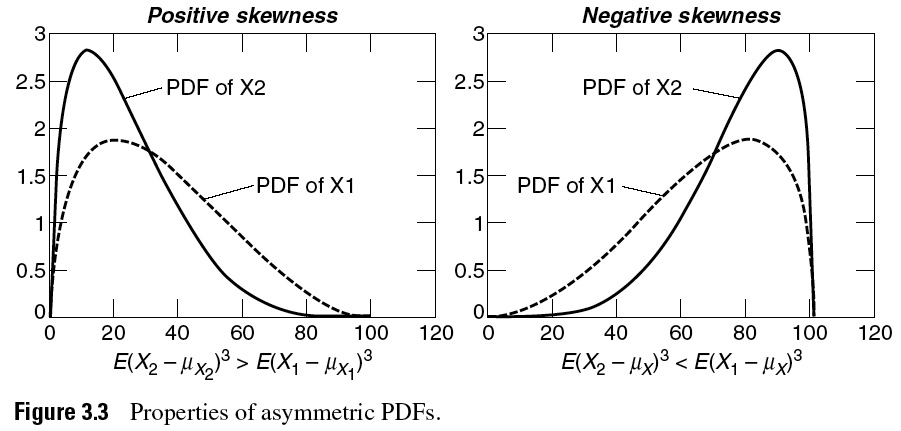
\includegraphics[width=\textwidth,trim={0 2cm 0 0},clip]{03_03}
  
% \end{frame}
% \begin{frame}
%   \frametitle{Kurtosis} \pause

%   This is the measure of peakedness in a distribution. \pause It is the fourth central moment: \pause

  
%   In the discrete case: \pause
%     \begin{equation}
%       \label{eq:8}
%       E(X - \mu_X)^4 = \sum_i(x_i - \mu_X)^4p_X(x_i)
%     \end{equation}
%     \pause

%     In the continuous case:\pause
%     \begin{equation}
%       \label{eq:6}
%       E(X - \mu_X)^4 = \int_{-\infty}^{\infty}(x - \mu_X)^4 f_X(x)dx
%     \end{equation}


% \end{frame}

% \begin{frame}
%   \frametitle{Skewness vs. kurtosis}
%   \pause

%   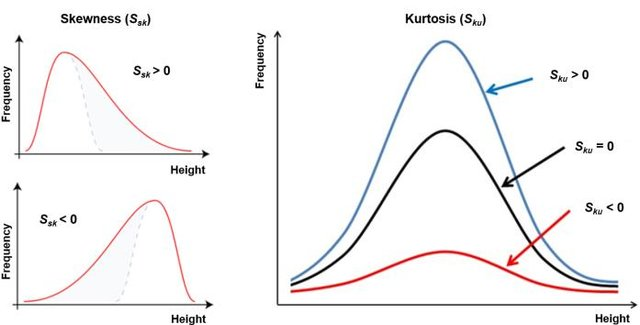
\includegraphics[width=\textwidth]{skewness-kurtosis}

%   {\tiny Source: Bonyar, A (2015) ``Application of localization factor for the detection of tin oxidation with AFM'' DOI: 10.1109/SIITME.2015.7342289}
% \end{frame}

% \begin{frame}
%   \frametitle{Generalized expectation}
%   The mathematical expectation can be defined for a function $g$ of random variable $X$:
  
%      \begin{align}
%       E[g(X)] &= \sum_i g(x_i) p_X(x_i) \quad \text{\og discrete case}\\ \pause
%       E[g(X)] &= \int_{-\infty}^{\infty}g(x)f_X(x)dx \quad \text{\og continuous case}
%     \end{align}

%   \end{frame}
  

%\backupend

%\begin{frame}[allowframebreaks]
%   \frametitle{References}
%   \AtNextBibliography{\scriptsize}
%   \setbeamertemplate{bibliography item}[text]
%   \printbibliography[heading=none]
  
% \end{frame}

%\printbibliography
\end{document}
%%% Local Variables:
%%% mode: latex
%%% TeX-master: t
%%% End:
